Betrachten Sie die folgenden Klassendiagrammkandidaten:

\figureSeriesHere{}{\figureSeriesRow{\figureSeriesElement{1}{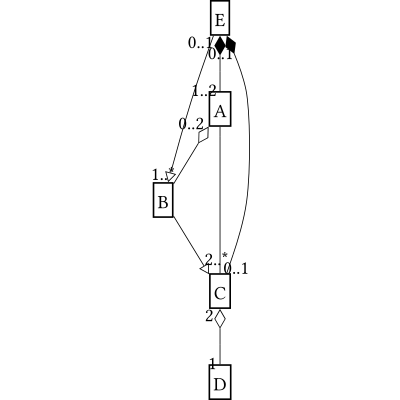
\includegraphics[min width=0.5\textwidth,min height=0.4\textwidth,max width=\textwidth,max height=\textwidth]{51/cdd1c5ae472de9a69c41400d40945817ce0c09750e9729e833d60a4440b740670400af83b04c596701db35357ce8aed00a3a92e08161.pdf}}}\figureSeriesRow{\figureSeriesElement{2}{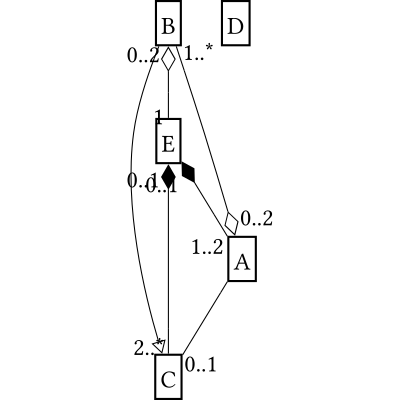
\includegraphics[min width=0.5\textwidth,min height=0.4\textwidth,max width=\textwidth,max height=\textwidth]{51/cd32786ed7955f75f2e4050d7464df637cf40075b2d129bb678089584e2eed975200af83b04c596701db35357ce8aed00a3a92e08161.pdf}}}\figureSeriesRow{\figureSeriesElement{3}{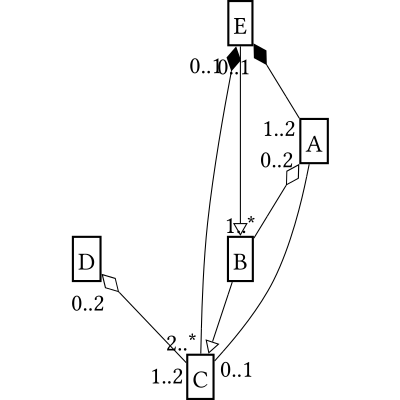
\includegraphics[min width=0.5\textwidth,min height=0.4\textwidth,max width=\textwidth,max height=\textwidth]{51/cdc2b5c869c289558f837f2bfe49d32b0e3b89293a325e08146a4a4c80b59e35fe00af83b04c596701db35357ce8aed00a3a92e08161.pdf}}}\figureSeriesRow{\figureSeriesElement{4}{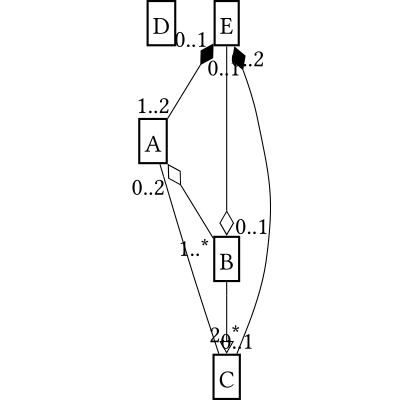
\includegraphics[min width=0.5\textwidth,min height=0.4\textwidth,max width=\textwidth,max height=\textwidth]{51/cd3faf14323c0cc9a0be4d24da2f2bee302bf2951cb8edca73b19f0e1599317b0300af83b04c596701db35357ce8aed00a3a92e08161.pdf}}}}Welche dieser Klassendiagrammkandidaten sind valide Klassendiagramme?
Bitte geben Sie Ihre Antwort in Form einer Liste von Zahlen an, die alle gültigen Klassendiagramme enthält.

Zum Beispiel würde
\begin{minted}{text}
[1, 2]
\end{minted}
bedeuten, dass nur die Klassendiagrammkandidaten 1 und 2 der angegebenen Klassendiagrammkandidaten gültige Klassendiagramme sind.

Bitte beachten Sie: Klassen werden hier vereinfacht dargestellt. 
 Das heißt, sie bestehen aus einer einfachen Box, die nur den Klassennamen enthält, aber keine Abschnitte für Attribute oder Methoden. 
 Trotzdem sollten Sie diese vereinfachten Klassendarstellungen als valide Klassen ansehen.

Bitte beachten Sie: Beim Bewegen über oder Klicken auf Kanten / Knoten bzw. ihre Beschriftungen werden die jeweils zusammengehörenden Komponenten hervorgehoben.

